\section{Diseño}

A continuación se muestra el diagrama de clases correspondiente al sistema generador 
de scorings.
\newline

\centerline{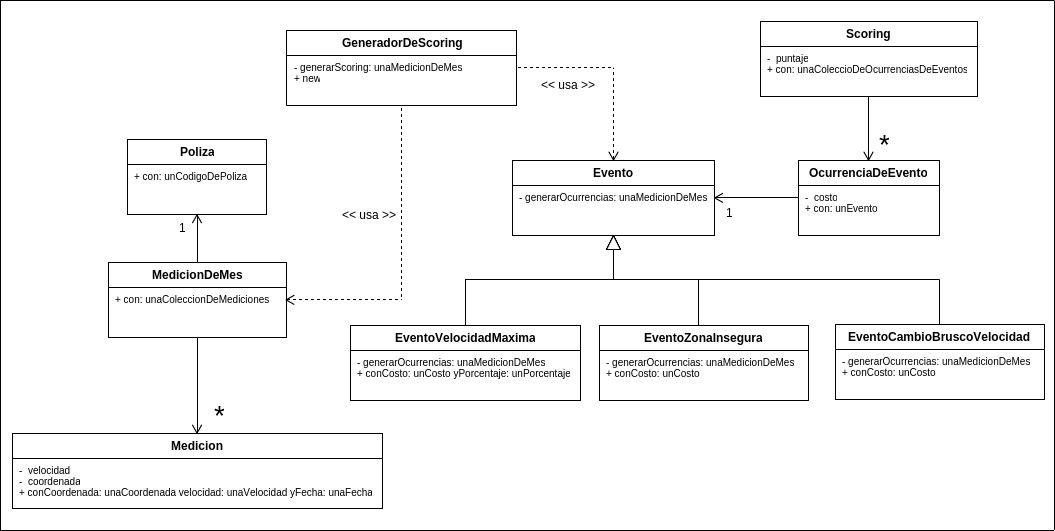
\includegraphics[width=1\textwidth]{./imagenes/clases.png}}


Como se ve en el diagrama, este diseño soporta el registro de distintos tipos de 
eventos. Se puede observar que en un futuro se podrán nuevos tipos de eventos 
sin hacer grandes modificaciones al modelo.




Debajo, se muestra el diagrama de secuencias del método \textit{generarScoring}.
La idea es mostrar como interactúa el \textit{Generador de Scoring} con los distintos
\textit{Eventos} para obtener el cojunto de \textit{Ocurrencias de Eventos}, utilizados
para calcular el scoring dada una \textit{Medición de Mes}. Esta última contiene las 
\textit{Mediciones} obtenidas durante cierto mes.
\newline

\centerline{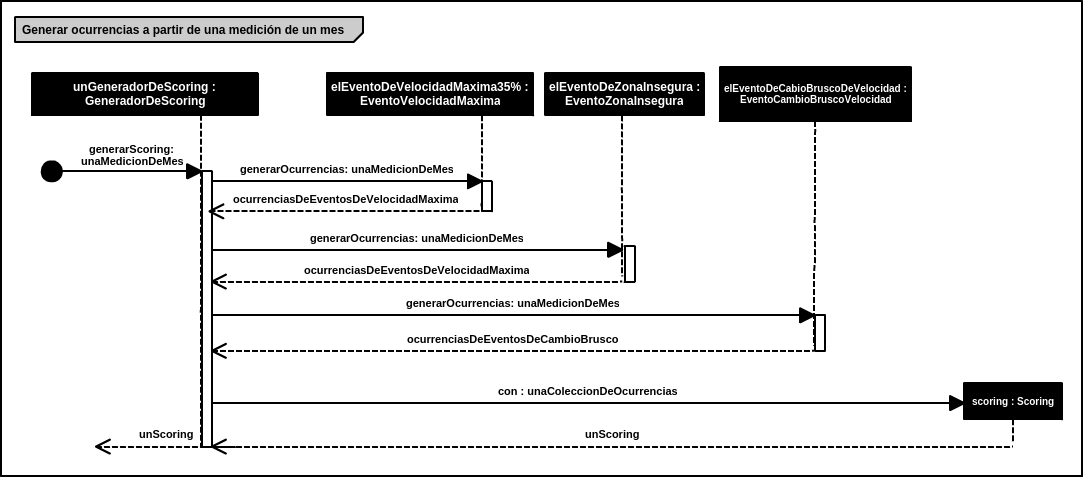
\includegraphics[width=1\textwidth]{./imagenes/secuencias_general.png}}

\newpage

Por otro lado, para complementar la idea explicada anteriormente, se presenta el diagrama
de objetos relacionado.


\centerline{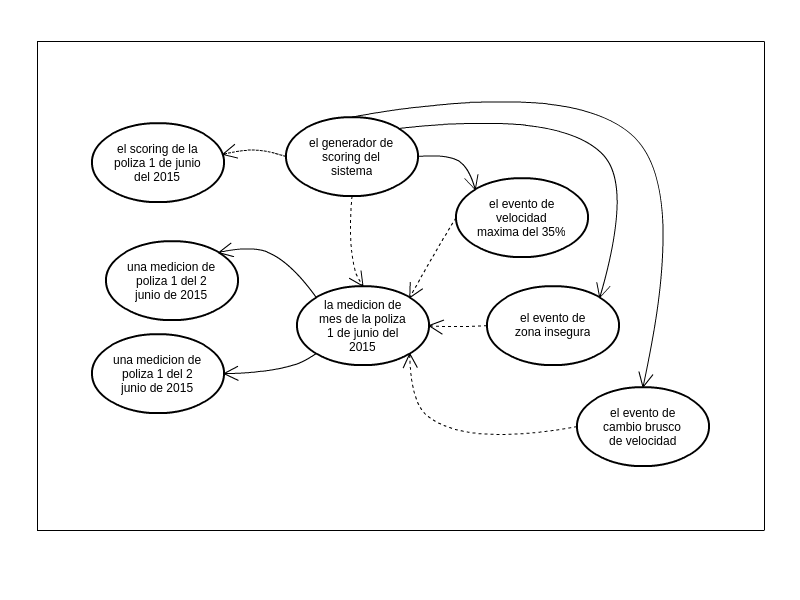
\includegraphics[width=1\textwidth]{./imagenes/objetos_general.png}}


Luego, para entrar más en detalle de cómo se crean las \textit{Ocurrencias de Eventos},
se realizó el diagrama de secuencias para el siguiente escenario:
\newline
- Dados una medición de mes con sólo una medición, la cual tiene una velocidad 50 km/h y una
coordenada en la cual la velocidad máxima es de 30 km/h, y un evento de velocidad máxima con 
un porcentaje de 10\%, se genera una ocurrencia de evento.
\newline


\centerline{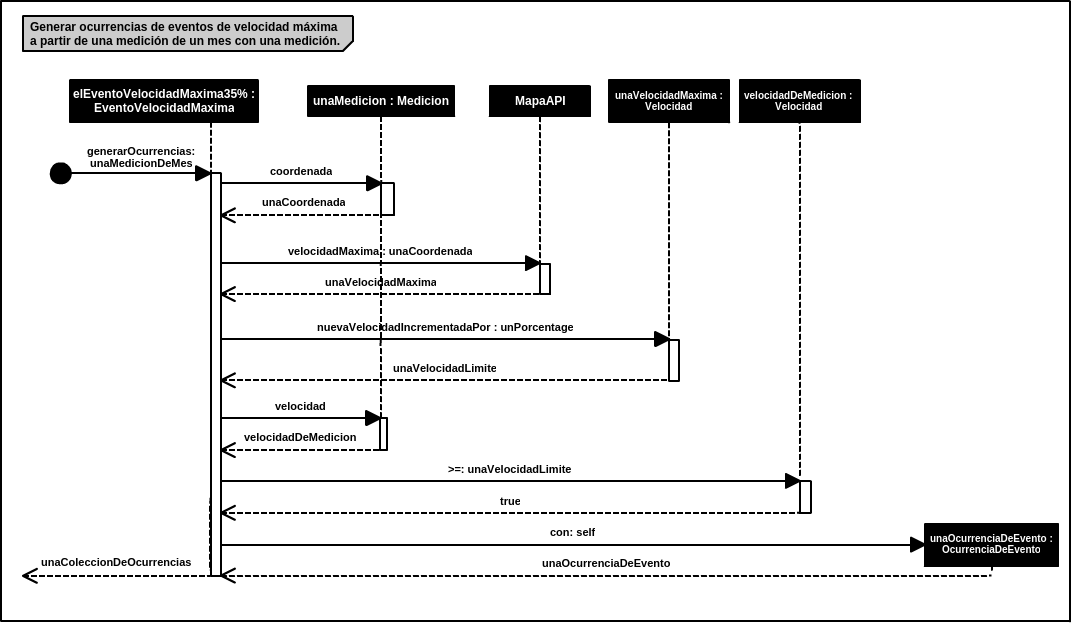
\includegraphics[width=1\textwidth]{./imagenes/secuencias_velmax.png}}


Aclaraciones:
\newline
- \textit{unPorcentaje} es el colaborador interno de \textit{elEventoDeVelocidadMaxima35\%}.
\newline
- En este diagrama, sólo se muestra el intercambio de mensajes con una medición pero esto se 
repetirá para cada medición del mes.



Para este escenario, también se realizó el diagrama de objetos:
\newline

\centerline{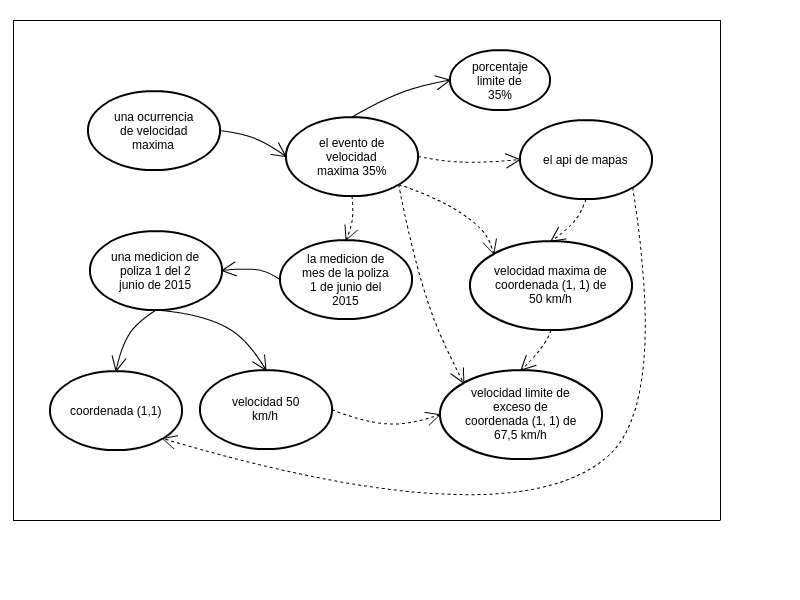
\includegraphics[width=1\textwidth]{./imagenes/objetos_velmax.png}}


\newpage
A continuación, se puede observar el diagrama de secuencias del siguiente escenario:\newline
- Dados una medición de mes con dos mediciones, con velocidades 60 km/h y 90 km/h, 
y un evento de cambio brusco de velocidad con una velocidad límite de cambio de 20 km/h, 
se genera una ocurrencia de evento.
\newline


\centerline{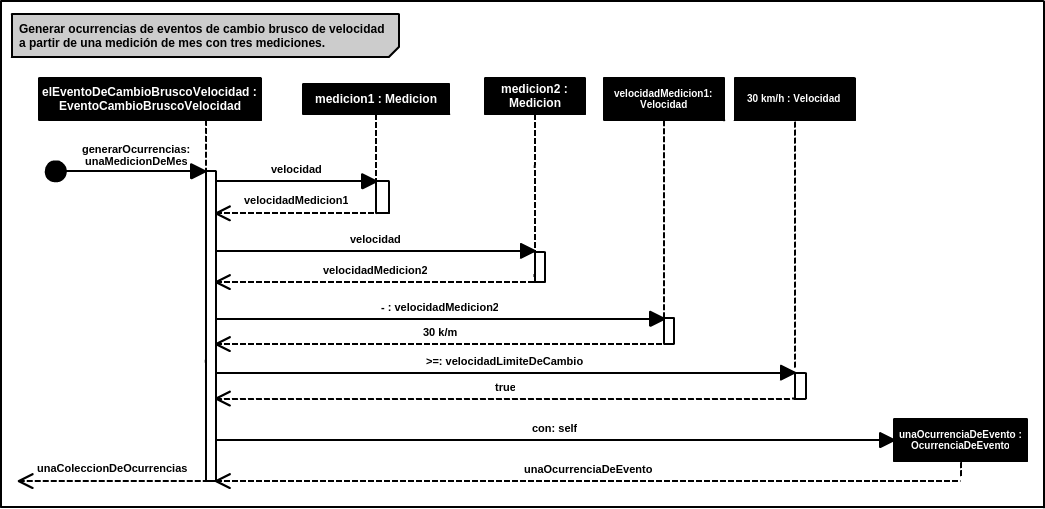
\includegraphics[width=1\textwidth]{./imagenes/secuencias_brusco.png}}


Aclaraciones:\newline
- La \textit{velocidadLimiteDeCambio} es colaborador interno de \textit{elEventoDeCambioBruscoVelocidad}\newline
- En este diagrama, sólo se muestra el intercambio de mensajes con un par de mediciones pero esto se 
repetirá para cada par de mediciones del mes.
